% This file was created by matplotlib2tikz v0.6.15.
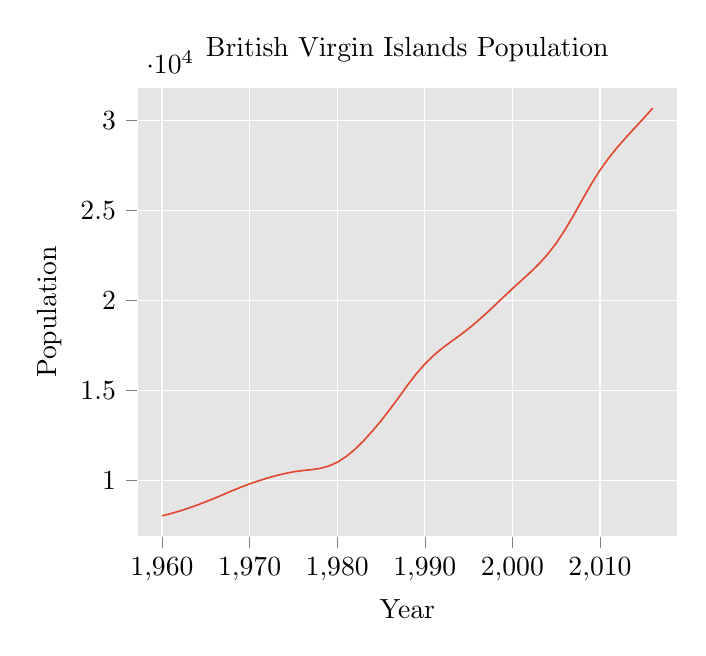
\begin{tikzpicture}

\definecolor{color0}{rgb}{0.886274509803922,0.290196078431373,0.2}

\begin{axis}[
title={British Virgin Islands Population},
xlabel={Year},
ylabel={Population},
xmin=1957.2, xmax=2018.8,
ymin=6901.6, ymax=31792.4,
tick align=outside,
tick pos=left,
xmajorgrids,
x grid style={white},
ymajorgrids,
y grid style={white},
axis line style={white},
axis background/.style={fill=white!89.80392156862746!black}
]
\addplot [semithick, color0, forget plot]
table {%
1960 8033
1961 8155
1962 8298
1963 8452
1964 8627
1965 8814
1966 9007
1967 9218
1968 9424
1969 9621
1970 9803
1971 9970
1972 10125
1973 10264
1974 10379
1975 10476
1976 10543
1977 10591
1978 10662
1979 10792
1980 11002
1981 11315
1982 11712
1983 12188
1984 12731
1985 13304
1986 13938
1987 14589
1988 15266
1989 15900
1990 16461
1991 16934
1992 17344
1993 17703
1994 18052
1995 18427
1996 18833
1997 19270
1998 19722
1999 20188
2000 20645
2001 21085
2002 21529
2003 22000
2004 22541
2005 23168
2006 23905
2007 24731
2008 25604
2009 26447
2010 27224
2011 27901
2012 28509
2013 29056
2014 29588
2015 30113
2016 30661
};
\end{axis}

\end{tikzpicture}